% --- SECTION 4 : INTRODUCTION AU GRADIENT FACTOR ---
\section{Paramétrage et Gradient Factors}

\begin{frame}{L'Ordinateur de Plongée — Réglages}
    L'ordinateur calcule la saturation en temps réel. Attention aux réglages avant la mise à l'eau :
    \begin{itemize}
        \item \textbf{Le Mélange} : Air ou Nitrox. \textit{\textcolor{ffessmred}{Danger} : Un ordi réglé sur Nitrox 
            pour une plongée à l'air indiquera moins de paliers que nécessaire}.
        \item \textbf{L'Altitude} : Au-dessus de 300m, les procédures changent (automatique ou manuel).
        \item \textbf{Les Alarmes} : Ne pas ignorer les alarmes sonores (vitesse de remontée, paliers).
        \item \textbf{La Dureté} : Possibilité de durcir les paliers pour plus de sécurité 
            (facteurs de risque).
    \end{itemize}
\end{frame}

\begin{frame}{Paramétrage — Durcissement des paliers}
    
    \begin{alertblock}{Quand durcir les paliers ?}
    \textbf{En cas de facteurs de risque :} \\
    fatigue, froid, effort important, successives rapprochées, etc.
    \end{alertblock}
    \begin{exampleblock}{Comment ?}
        \textbf{Réglages du conservatisme selon les modèles :}
        \begin{itemize}
            \item \textbf{Modèles Bühlmann (Scubapro, Uwatec) :} Niveau L0 à L5 de microbulles.
            \item \textbf{Modèles RGBM (Suunto, Cressi, Mares) :} Conservatisme niveaux 0 à 2.
            \item \textbf{Modèles Suunto-fused RGBM (Eon, DX) :} Conservatisme niveau -2 à niveau +2.
            \item \textbf{Gammes Oceanic et Beuchat :} Conservatisme Off ou On.
        \end{itemize}
    \end{exampleblock}
\end{frame}

\begin{frame}{Le Gradient Factor (GF) : Durcir sa sécurité}
    \begin{itemize}
        \item \textbf{Définition :} Paramètre permettant de "durcir" l'algorithme de décompression (souvent Bühlmann) pour prendre plus de marge.
        \item \textbf{Pourquoi ?} Pour s'adapter à sa forme, son âge ou aux conditions (froid, fatigue).
        \item \textbf{GF Bas / GF Haut :}
        \begin{itemize}
            \item \textit{GF Bas :} Définit la profondeur du premier palier.
            \item \textit{GF Haut :} Définit la quantité d'azote résiduel acceptée en surface.
        \end{itemize}
    \end{itemize}
    \begin{alertblock}{Réglage ordinateurs "loisir"}
        Sur beaucoup d'ordinateurs "loisir", cela correspond aux modes de sécurité \textbf{SF} (Safety Factor) ou \textbf{P} (Personalization) de 0 à 2.
    \end{alertblock}
\end{frame}

\begin{frame}{Le Gradient Factor (GF) : Sans marge de sécurité}
    \begin{columns}
        \column{0.5\textwidth}
        \begin{center}
            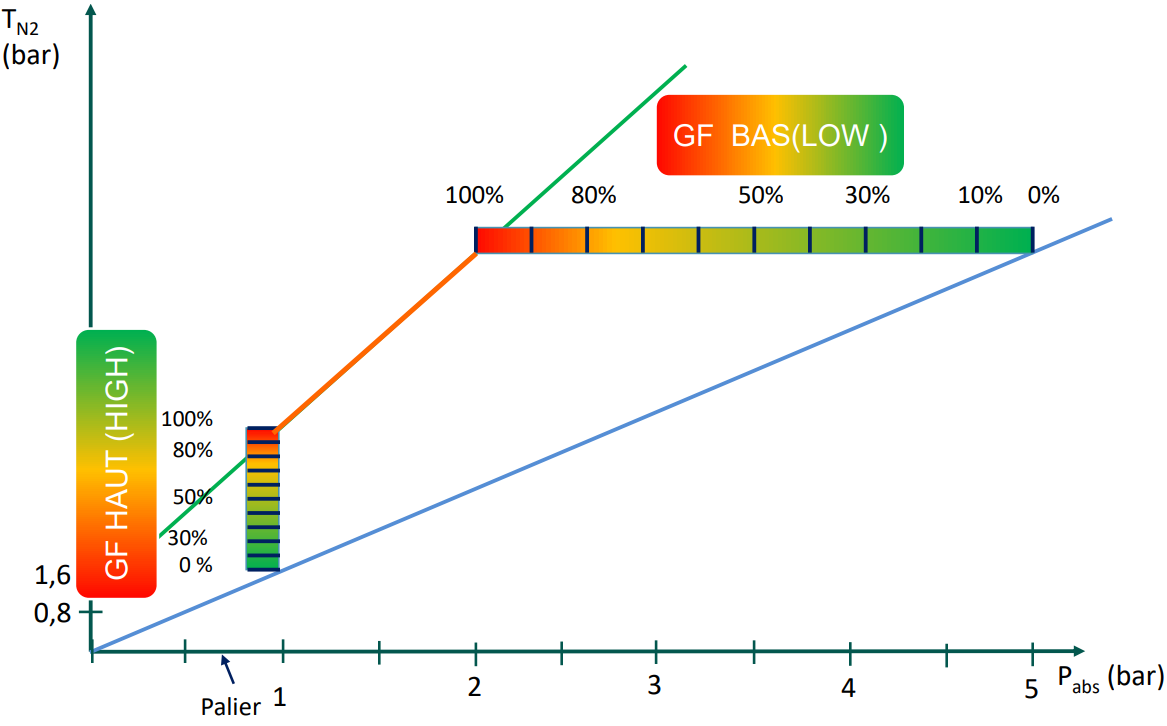
\includegraphics[width=\textwidth]{images/gf_100_100}
        \end{center}
        \column{0.45\textwidth}
        \begin{itemize}
            \item \textbf{Ligne verte} : Limite de sécurité absolue.
            \item \textbf{GF 100/100} : Modèle pur sans marge.
            \item \textbf{GF Bas} : Règle votre premier palier.
            \item \textbf{GF Haut} : Sécurité proche de la surface.
            \item \textbf{Réduire \%} : Augmente votre marge d'erreur.
            \item \textbf{Objectif} : Limiter la création de bulles.
        \end{itemize}
    \end{columns}
\end{frame}

\begin{frame}{Le Gradient Factor (GF) : GF 85/85}
    \begin{columns}
        \column{0.5\textwidth}
        \begin{center}
            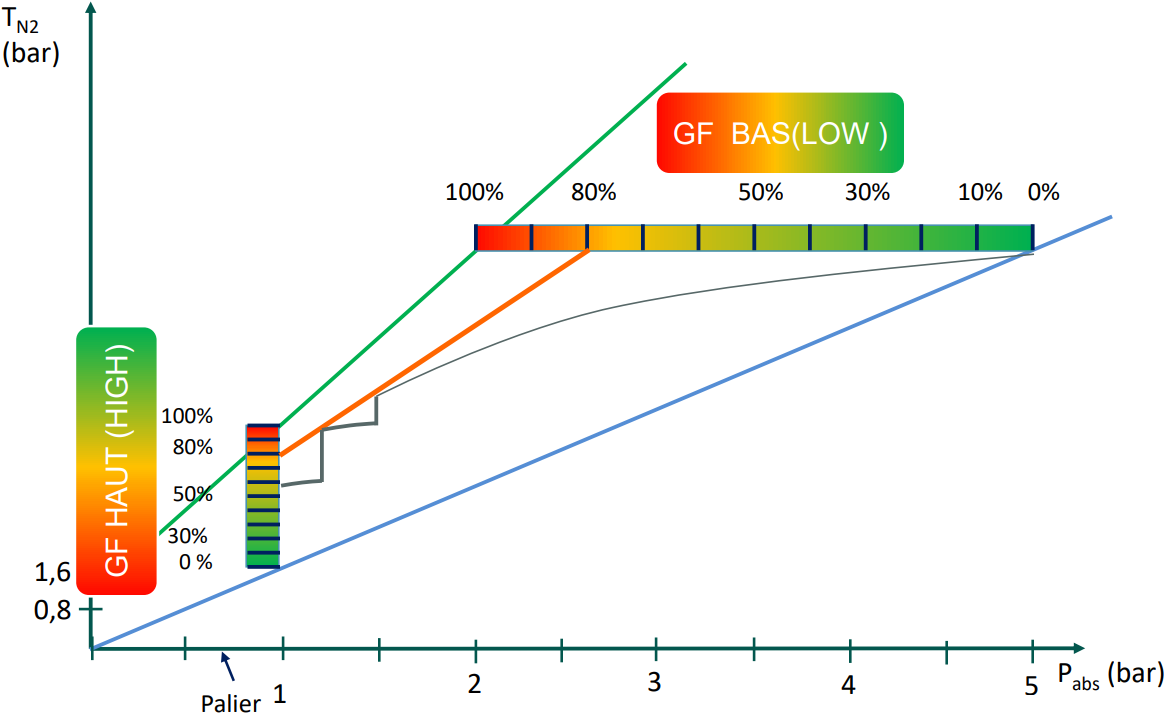
\includegraphics[width=\textwidth]{images/gf_85_85}
        \end{center}
        \column{0.45\textwidth}
        \begin{itemize}
            \item \textbf{Réglage 85/85} : 15\% de marge de sécurité.
            \item \textbf{Moins de \%} : Moins de bulles, plus de paliers.
        \end{itemize}
        \begin{block}{Conclusion}
            \textbf{GF 85/85} : Un bon compromis pour la plupart des plongeurs, et conseillé par la FFESSM.
        \end{block}
    \end{columns}
\end{frame}

\begin{frame}{Le Gradient Factor (GF) : GF 30/70}
    \begin{columns}
        \column{0.55\textwidth}
        \begin{center}
            \begin{tikzpicture}
                \node[anchor=south west, inner sep=0] (image) at (0,0) {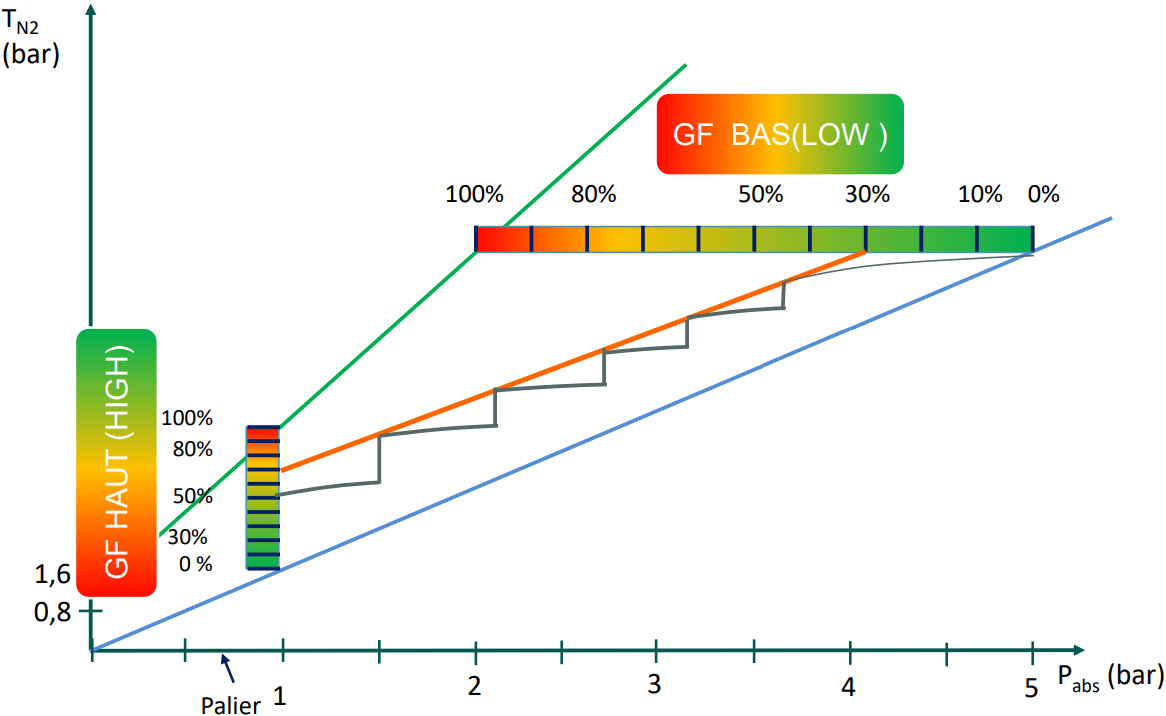
\includegraphics[width=\textwidth]{images/gf_30_70}};
                
                \node[font=\bfseries\small, align=center, text=red] (legende) at (5, 1.2) {1\textsuperscript{er} palier \\ profond};

                \draw[<- , >=latex, red, very thick] (5.65, 2.95) -- (legende.north);
            \end{tikzpicture}
        \end{center}
        \column{0.45\textwidth}
        \begin{itemize}
            \item \textbf{Réglage 30/70} : 30\% à 40\% de marge.
            \item \textbf{Effet} : Paliers plus profonds et longs.
            \item \textbf{Risque à l'air} : Continue de saturer les tissus lents.
            \item \textbf{Origine} : Plongée technique (Trimix).
        \end{itemize}
        
        \begin{alertblock}{Conclusion}
            \textbf{GF 30/70} : Inadapté à l'air. Favorise la saturation au lieu de la désaturation.
        \end{alertblock}
    \end{columns}
\end{frame}
